\documentclass{article}

\usepackage{amsmath}
\usepackage{amsfonts}
\usepackage{amssymb}
\usepackage{graphicx}
\graphicspath{{./images/}}

\usepackage[
  backend=biber,
  style=apa,
  citestyle=apa
]{biblatex}
\addbibresource{references.bib}

\title{A Simple Housing Price Transmission Mechanism for Monetary Policy}
\author{Emmet Hall-Hoffarth}
\date{\today}

\begin{document}
\maketitle
    
\section{Setup}

Assume an endowment economy in which a unit mass of overlapping generations of agents live for two periods denoted $t$ and $t+1$ and possess initial wealth uniformly distributed over the unit interval such that $\omega_{it} \sim U(0,1)$. There are two types of agents, homeowners and renters. I will assume that renter agents can only save in cash, and are therefore subject to uninsurable inflation risk. Homeowner agents on the other hand can invest in housing (on which they must pay interest, but may benefit from the appreciation of) or in an interest-bearing bond. Thus, the homeowner agents are strictly better off than the renter agents. Both types of agents derive utility from and therefore have demand for consumption goods and housing. For simplicity, I will not yet model the supply side of the economy. In both periods the aggregate supply of consumption goods and housing is $1$\footnote{To get the important results here we could have any supply for consumption goods as long as steady state production is 1. On the other hand, housing supply does need to be fixed, however, this is likely a reasonable approximation of housing supply, at least in the short run.}. Homeowner agents will be able to satisfy their demand for housing by purchasing a housing asset at price $p^a_t$ when they are young that they can then sell in period next period when they are old. Renters on the other hand will have to rent their housing at price $r^a_t$. In period $t+1$ both types agents born in period $t$ will rent at price $r^a_{t+1}$ to fulfil their housing demand. All renters will rent from the (young) homeowner agents, and occupy the housing that the homeowners themselves do not.

The key complexity of this model is that the type of agents is determined endogenously in equilibrium. Agents will become renters if their wealth is below $\phi p^a_t$ for some constant $0 < \phi < 1$. Given the distributional assumption about wealth, this is also equal to the mass of agents who are renters. The rest of the agents are homeowners. The real life phenomenon that this is meant to represent is a minimum down-payment that must be made to obtain a mortgage. The aim of the model is to show that if monetary policy today prices some agents out of the housing market, it may have implications for monetary policy in the future, since renter agents are less sensitive to monetary policy decisions.

\section{Renter Problem}

Consider first the optimization problem of renter agents, which is fairly trivial. Assume that both types of agents have utility of the form $U(c, a) = ln(c) + ln(a)$, and normalize the price of consumption good in period $t$ ($p_t$) to $1$. I adopt the following notation: $c^r_{t+1|t}$ is the consumption of renter agents (r) in period $t+1$ who were born in period $t$ (when they are old). The renter agents solve:

\begin{align}
    \underset{c^r_{t|t}, c^r_{t+1|t}, a^r_{t|t}, a^r_{t+1|t}, \omega_{t+1|t}}{\max} &ln(c^r_{t|t}) + ln(a^r_{t|t}) + \beta[ln(c^r_{t+1|t}) + ln(a^r_{t+1|t})] \nonumber \\
    \text{s.t. }& \omega_{t|t} = c^r_{t|t} + r_{t|t}^a a^r_{t|t} + \omega_{t+1|t} \nonumber \\
    & \omega_{t+1|t} = \mathbb{E}_t(p_{t+1})c^r_{t+1|t} + \mathbb{E}_t(r^a_{t+1})a^r_{t+1|t}
\end{align}

The resulting optimality conditions combined with the wealth of renter agents results in the following equilibrium conditions:

\begin{align}
    c^r_{t|t} = r^a_t a^r_{t|t} =& \frac{\phi p^a_t}{2(1+\beta)} \label{renter_optimal_{t|t}} \\
    \mathbb{E}_t(p_{t+1}) c^r_{t+1|t} = \mathbb{E}_t(r^a_{t+1}) a^r_{t+1|t} =& \frac{\beta \phi p^a_t}{2(1+\beta)} \label{renter_optimal_{t|t}1}
\end{align}

When log-linearized these yield:

\begin{align}
    \hat{c}^r_{t+1|t} =& (1-\mathbb{E}_t(\pi_{t+1|t}))\hat{c}^r_{t|t} \\
    \hat{a}^r_{t+1|t} =& (1-\mathbb{E}_t(\pi^r_{t+1|t}))\hat{a}^r_{t|t} \\
    \hat{c}^r_{t|t} =& \hat{r}^a_{t|t} + \hat{a}^r_{t|t}
\end{align}

\section{Homeowner Problem}

Now consider the optimization problem of homeowner agents. They solve:

\begin{align}
    &\underset{c^o_{t|t}, c^o_{t+1|t}, a^o_{t|t}, a^i_{t|t} a^o_{t+1|t}, b_{t|t}}{\max} ln(c^o_{t|t}) + ln(a^o_{t|t}) + \beta[ln(c^o_{t+1|t}) + ln(a^o_{t+1|t})] \nonumber \\
    \text{s.t. }& \omega_{t|t} + r^a_t(a^i_{t|t} - a^o_{t|t}) = c^o_{t|t} + p^a_t (1 + i_t) a^i_{t|t} + b_{t|t} \nonumber \\
    & (1 + i_t) b_{t|t} + \mathbb{E}_t (p^a_{t+1}) a^i_{t|t} = \mathbb{E}_t(p_{t+1})c^o_{t+1|t} + \mathbb{E}_t(r^a_{t+1})a^o_{t+1|t}
\end{align}

Where $a^i_{t|t}$ is the amount of housing purchased (invested in) by homeowners, and $a^o_{t|t}$ is the amount of housing actually lived in (consumed) by homeowners. Note that it will be assumed that bond holdings are zero in equilibrium. The threat of bond owning is sufficient to impose a no-arbitrage condition. Also note that the homeowners can either live in their home and extract utility, or they can rent it on the housing market. This problem implies the following first order conditions:

\begin{align}
    \lambda_{t+1|t} =& \frac{\lambda_{t|t}}{1+i_t} = \frac{\beta}{\mathbb{E}_t(r^a_{t+1}) a^o_{t+1|t}} \label{ho_multiplier} \\
    c^o_{t|t} =& r^a_t a^o_{t|t} \label{ho_intertemporal} \\
    \frac{r^a_t}{p^a_t} +& \frac{\mathbb{E}_t(\Pi^a_{t+1|t})}{1+i_t} = 1+ i_t \label{no_arb} \\
    c^o_{t+1|t} =& \beta \frac{1 + i_t}{\mathbb{E}_t (p_{t+1})} c^o_{t|t} \label{ho_euler} \\
    a^o_{t+1|t} =& \beta \frac{1+i_t}{\mathbb{E}_t(\Pi^r_{t+1|t})} a^o_{t|t} \label{ho_hous_euler}
\end{align}

The first condition pins down both of the multipliers as a function of the housing choice. The second condition is equivalent to the consumption-housing decision for the renter agent. This is because although the homeowner agent does not pay rent it is still the opportunity cost for them to live in the housing they own. The third condition can be interpreted as a no-arbitrage condition. The left-hand side is the expected return of investing in a marginal unit of housing, and the right-hand side is the return on a marginal unit of bonds. The final two conditions are Euler equations for consumption and housing. When log-linearized these Euler equations yield:

\begin{align}
    \hat{c}^o_{t+1|t} =& (1 + \hat{i}_{t|t} - \mathbb{E}_t(\pi_t))\hat{c}^o_{t|t} \\
    \hat{a}^o_{t+1|t} =& (1 + \hat{i}_{t|t} - \mathbb{E}_t(\pi^r_t))\hat{a}^o_{t|t} \\
\end{align}

\section{Equilibrium}

In order to fully understand the aggregate dynamics we need to pin down the steady-state housing price. To do this, we will employ the optimality conditions along with the aggregate resource constraints. We will assume that total supply of consumption goods and housing in the economy is 1 in every period. This implies that $a^i_{t|t} = 1$.  Given that in any given period there is a young generation and an old generation, each of which contains both types of agents, the aggregate resource constraints read:

\begin{align}
    c^r_{t+1|t} + c^o_{t+1|t} + c^r_{t+1|t} + c^o_{t+1|t} = y_{t+1} = 1 \label{consumption_rc} \\
    a^r_{t+1|t} + a^r_{t+1|t} + a^o_{t+1|t} = a^i_{t+1|t+1} - a^o_{t+1|t+1} = 1 - a^o_{t+1|t+1} \label{housing_rc}
\end{align}

In steady state all prices are constant so in particular it follows that $\mathbb{E}_t(\Pi_{t+1|t}) = \mathbb{E}_t(p_{t+1}) = \mathbb{E}_t(\Pi^a_{t+1|t}) = 1$ and $\mathbb{E}_t({r^a_{t+1}}) = r^a_t = \bar{r}^a$. After combining this steady state assumption with the aggregate resource constraint and optimality conditions, further simplifications yield:

\begin{equation}
    \bar{p}^a = \frac{1 + \bar{i}}{\bar{i}(1 + \beta(1 + \bar{i}))} \label{ss_housing_price}
\end{equation} 

Which indeed implies that $\bar{p}^a$ is a decreasing function of $\bar{i}$\footnote{I am working on an extension where the homeowners only pay interest on the amount invested in housing that is above the down payment. This will make $\bar{p}^a$ depend on $\phi$ as it currently does not, however, it does not change any of the qualitative results.}. In particular, $\bar{p}^a$ goes to infinity as $\bar{i}$ goes to zero and vice-versa. Therefore, as the steady state policy rate decreases so too does the proportion of agents who are homeowners. Note that since we originally assumed that $0 < \phi p^a_t < 1$ this does imply a parameter restriction relating $\bar{i}$ and $\phi$. If $\phi$ is too high relative to $\bar{i}$ then this can imply that no agents are homeowners, and this breaks down the equilibrium\footnote{I foresee an extension here where a fiscal authority is in charge of $\phi$, and in accordance to the logic here they are likely to select a lower $\phi$ in low interest regimes. This would for example be the case if they chose $\phi$ to keep the proportion of homeowners constant. With some extension to the model to allow for such a thing to exist, this would make financial instability more likely in such a circumstance.}. This constraint is relatively mild under reasonable assumptions, but it does mean that this model is not valid in very low or zero interest regimes. We can then combine the log-linear optimality conditions for both types of agents in order to elucidate the aggregate dynamics of output in the model. Doing so we obtain:

\begin{align}
    \hat{c}_{t+1} =& (1-\frac{1}{2} \phi \bar{p}^a)(1 +\hat{i} - \mathbb{E}_t (\pi_{t+1})) \hat{c}^o_{t|t} \nonumber \\
    +& \frac{\beta \phi \bar{p^a}}{2(1+\beta)} (1 - \mathbb{E}_t(\pi_{t+1})) \hat{c}^r_{t|t} \nonumber \\
    +& \frac{1-\frac{1}{2} \phi \bar{p}^a}{1 + \beta(1+\bar{i})} \hat{c}^o_{t+1|t+1} \nonumber \\
    +& \frac{\phi \bar{p^a}}{2(1+\beta)} \hat{c}^r_{t+1|t+1} \label{is_equation}
\end{align}

This is the IS equation for this economy, and it illustrates the primary mechanism of this model. The coefficient on each term is the proportion of each type of agent in the steady state of the economy, and we can see from this the proportion of homeowner agents in the economy is inversely related to $\bar{p}^a$, and therefore positively related to $\bar{i}$. The consumption decision of agents who are renters is not directly affected by changes to the nominal rate, only through general equilibrium. On the other hand, homeowner agents have a standard New Keynesian IS curve, and will substitute intertemporally accordingly. Therefore, in a regime where the steady state level of the policy rate is lower, the impulse response to an otherwise equivalent monetary policy shock will be relatively weaker.

In the current setting such deviations in consumption are must be zero-sum because production is fixed. Thus, monetary policy shocks can only actually result in redistribution. However, the IS equation in principle reflects the change in relative demand for consumption goods, and thus is indicative of how aggregate output would evolve if it were not fixed. However, extending the model in order to allow for production to respond continuously to changes in demand by adding a New Keynesian production side to the economy, while maintaining analytical tractability, seems to be impossible. While under such assumptions it may still be possible to characterize a steady-state --- indeed, if steady state production is equal to unity all of the proceeding results are unaffected --- the real purpose of such modelling would be to explore the dynamic reaction of the system to shocks, and this is infeasible even insofar as log-linearization can be employed.

This is because in even a very simple production side where labour is the only input, in order for output to respond to demand the labour supply must also be flexible and hence endogenously determined by the agent. This is problematic because each agent may then manipulate their labour supply choice in order to affect which side of the cut-off they fall on. This in turn depends on the relative utility value which itself again depends upon the cut-off. So adding endogenous labour choice this model adds yet another layer of equilibrium logic to what is already a highly non-linear model with second order equilibrium effects\footnote{In the baseline model the first-order effect of a monetary policy shock is the effect on demand (IS curve). The second order effect is the effect on the distribution of agents through its impact on asset prices, and hence the relative composition of each agent type in demand. In this view adding endogenous labour supply results in a third-order effect whereby the second-order effect causes a further change to output via the hetergenous labour supply choice.}.

\begin{appendix}
\section{Proof of (\ref{ss_housing_price})}

In steady state (\ref{no_arb}) implies:

\begin{equation}
    \bar{p}^a = \frac{1+\bar{i}}{(1+\bar{i})^2 - 1}\bar{r}^a \label{ss_no_arb}
\end{equation}

The consumption and housing of each of the four types of agents (young or old, renter or homeowner) are also constant, but they are not necessarily the same as that of any other type. We will now utilize the first order conditions and resource constrains in steady state to derive a second equation relating $\bar{p}^a$ and $\bar{r}^a$. In steady state, (\ref{renter_optimal_{t|t}}), (\ref{renter_optimal_{t|t}1}), (\ref{ho_euler}), and (\ref{consumption_rc}) imply:

\begin{align}
    & (1+\beta)\frac{\phi\bar{p}^a}{2(1+\beta)} + (1+\beta(1+\bar{i})) \bar{c}^o_{t|t} = 1 \nonumber \\
    \implies& \bar{c}^o_{t|t} = \frac{2-\phi\bar{p}^a}{2(1+\beta(1+\bar{i}))} \label{ss_ho_opt_cons}
\end{align}

Where $\bar{c}^o_{t|t}$ refers to the steady-state consumption of a homeowner agent born in the current period. The first order conditions (\ref{ho_intertemporal}) and (\ref{ho_hous_euler}) the homeowner agent imply:

\begin{align}
    & \bar{a}^o_{t|t-1} = \frac{\beta(1+\bar{i})}{\bar{r}^a} \bar{c}^o_{t|t} \\
    \text{(\ref{ss_ho_opt_cons})} \implies& \bar{a}^o_{t|t-1} = \frac{\beta(1+\bar{i})(2-\phi\bar{p}^a)}{2\bar{r}^a(1+\beta(1+\bar{i}))} \label{ss_ho_opt_hous1}
\end{align}

Combining (\ref{ss_ho_opt_hous1}) with (\ref{housing_rc}) we obtain:

\begin{align}
    1-\bar{a}^o_{t|t} =& (1+\beta) \frac{\phi \bar{p}^a}{2(1+\beta)\bar{r}^a} + \frac{\beta(1+\bar{i})(2-\phi\bar{p}^a)}{2\bar{r}^a(1+\beta(1+\bar{i}))} \nonumber \\
    \bar{a}^o_{t|t} =& 1 - \frac{2(1+\bar{i})+\phi \bar{p}^a}{2\bar{r}^a(1+\beta(1+\bar{i}))} \label{ss_ho_opt_hous}
\end{align}

Finally, (\ref{ho_hous_euler}), (\ref{ss_ho_opt_hous}), and (\ref{ss_ho_opt_hous1}) imply:

\begin{align}
    \frac{\beta(1+\bar{i})(2-\phi\bar{p}^a)}{2\bar{r}^a(1+\beta(1+\bar{i}))} =& \beta (1+\bar{i}) \left(1 - \frac{2(1+\bar{i})+\phi \bar{p}^a}{2\bar{r}^a(1+\beta(1+\bar{i}))}\right) \nonumber \\
    \implies \bar{r}^a =& \frac{2+\bar{i}}{1+\beta(1+\bar{i})} \label{ss_r}
\end{align}

Then (\ref{ss_housing_price}) follows from combining (\ref{ss_no_arb}) and (\ref{ss_r}) $\square$

\section{Plot of Steady State Housing Price}

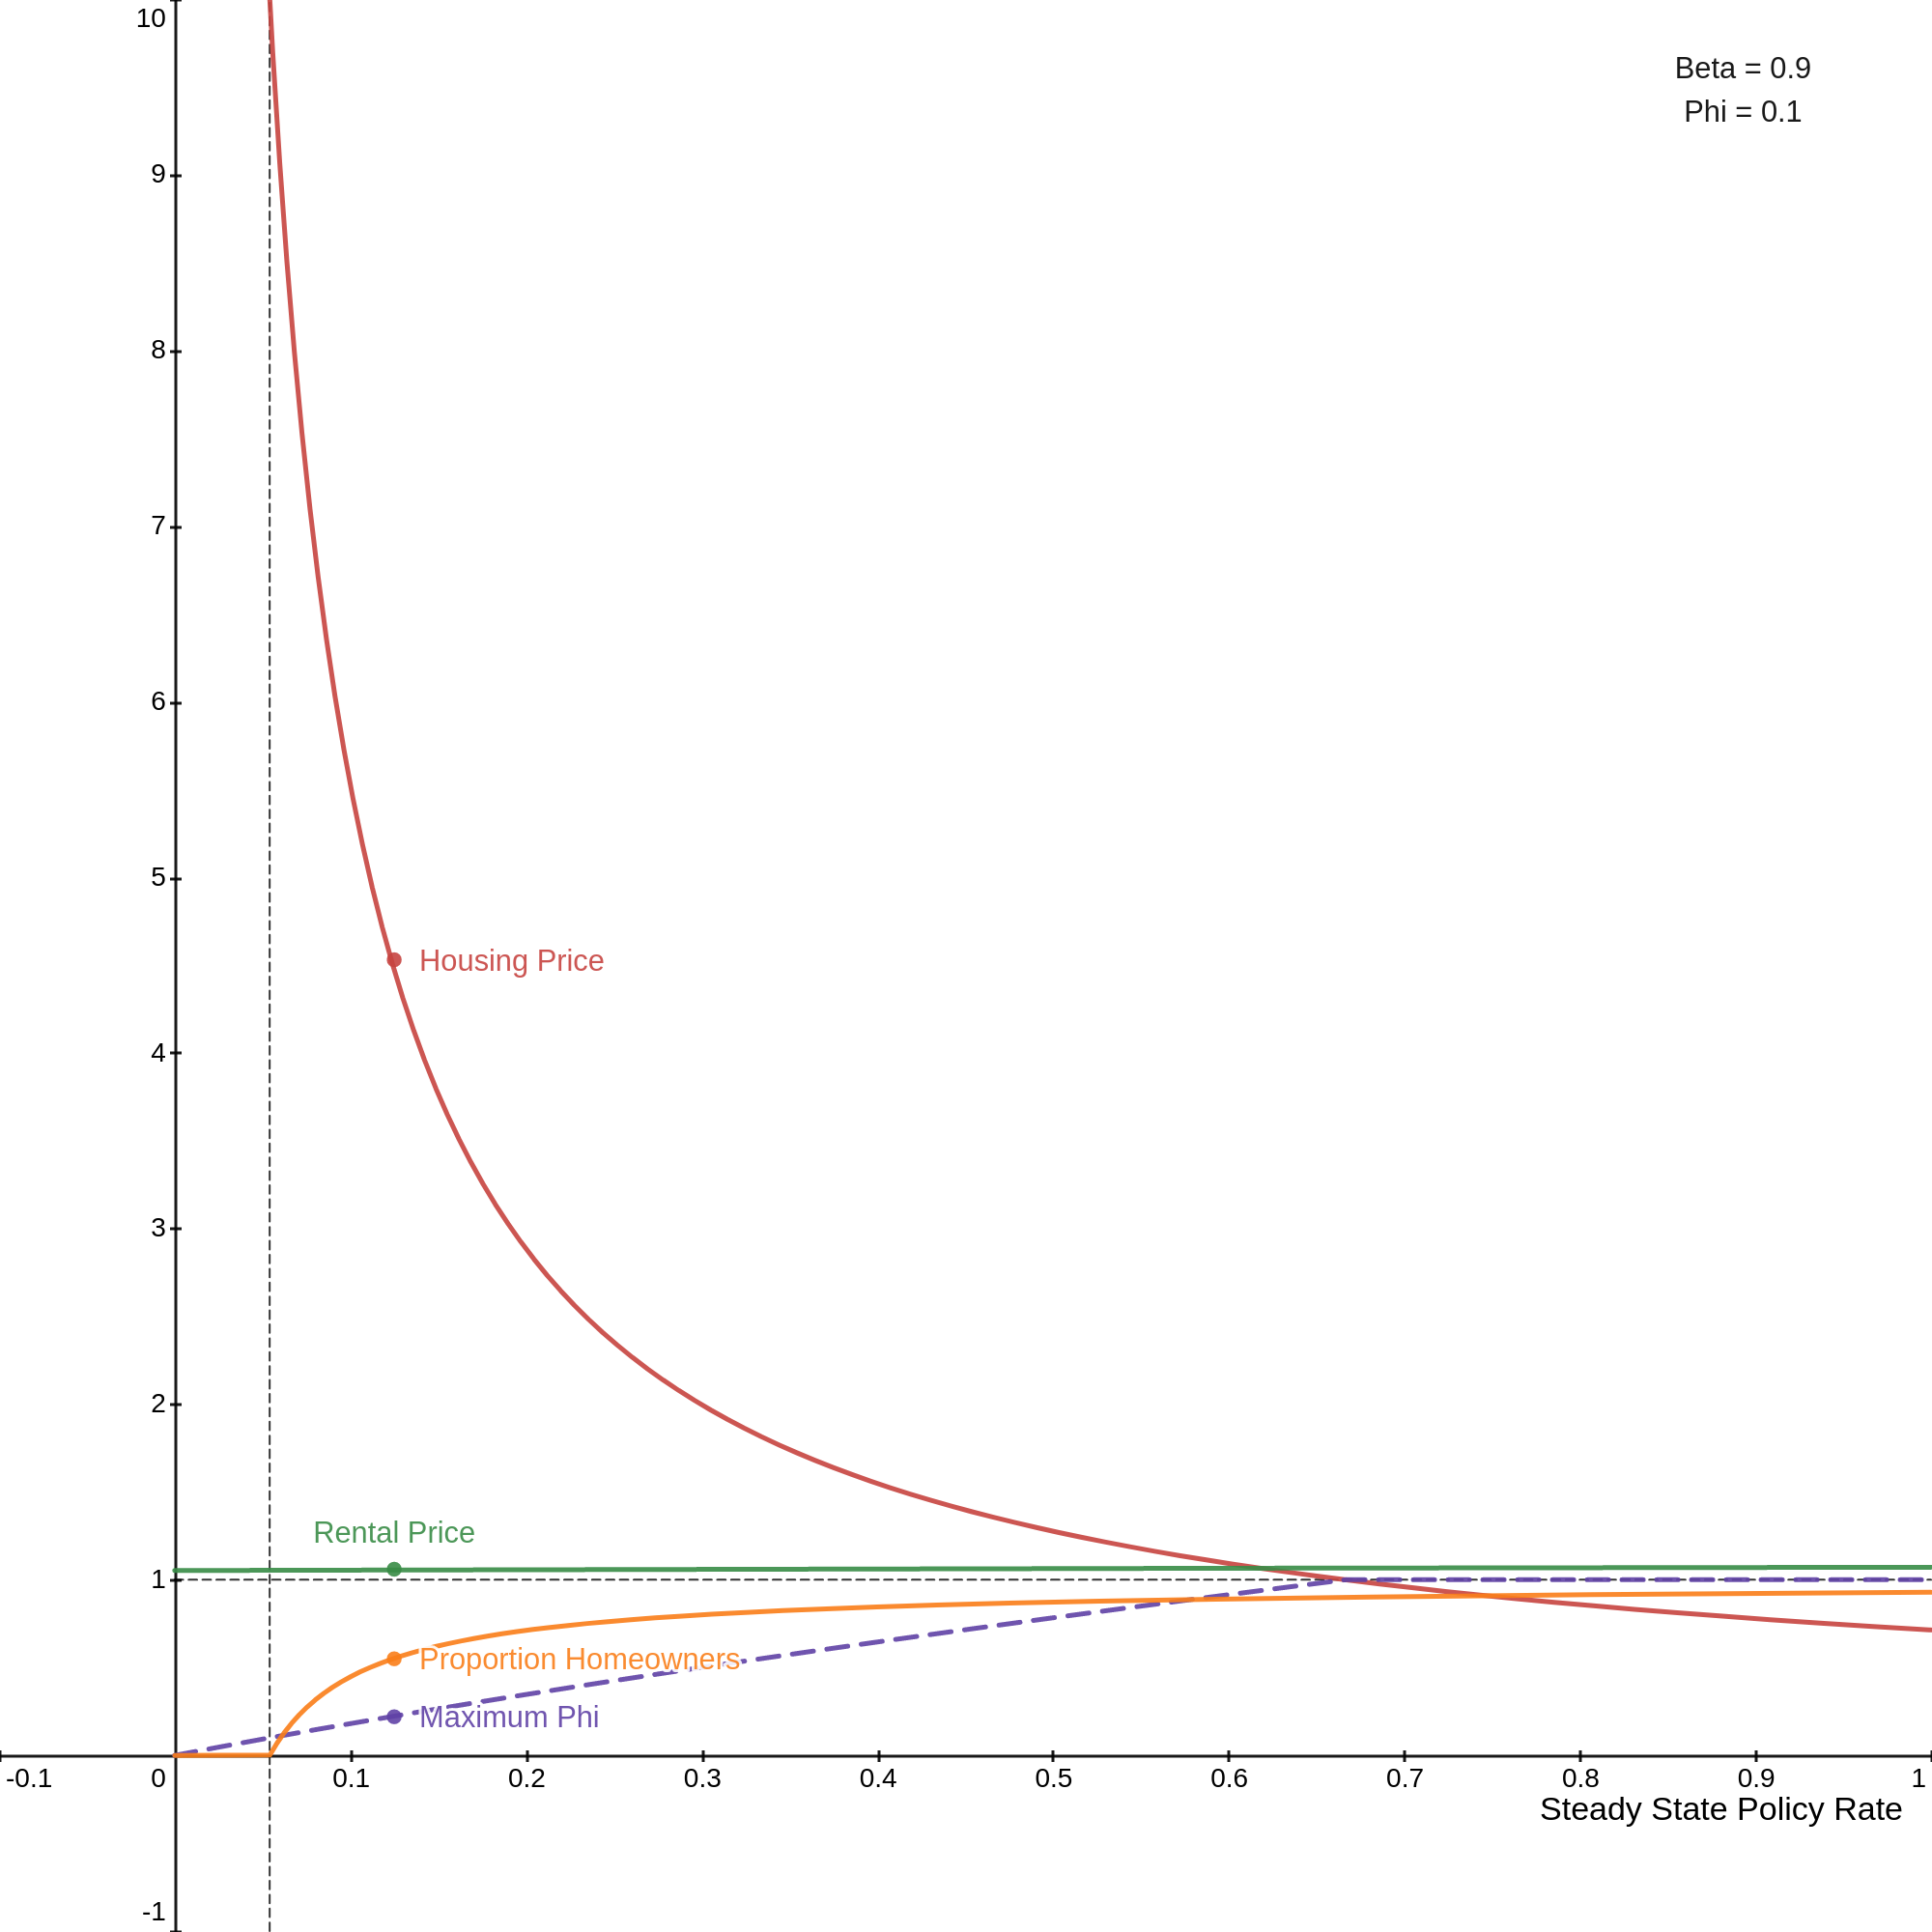
\includegraphics[width=\linewidth]{asset_price_rental_rate.png}

\end{appendix}

\end{document}